\chapter{Results}
\label{ch:results}
This chapter presents an evaluation of the algorithms introduced in Chapter \ref{ch:heuristics}.
To assess their performance, a cumulative distribution plot was used.
This type of plot shows the percentage of instances for which an algorithm found a plan with a
primal gap below the threshold indicated on the x-axis.
The best algorithm is the one whose curve lies above all the others.
The plots presented in the following sections will help illustrate this concept.
As described in Chapter \ref{ch:methodology}, each algorithm was run on every instance in the
testbed 10 times, each with a different random seed.
There are 3,104 instances, so each algorithm was executed a total of 31,040 times.
To limit execution time, each run was given a time limit of 60 seconds. The instances
come from different domains; some are very large in terms of number of actions, while others are
relatively small.
Additionally, since some algorithms are more efficient than others, not all the instances
were solved by every algorithm. Table \ref{tab:timelimit} shows, for each algorithm,
the number of instances it was able to solve within the time limit.

\begin{table}[ht]
	\centering
	\begin{tabular}{|l|r|}
		\hline
		\textbf{Heuristic}        & \textbf{Not found per timelimit} \\
		\hline
		Random                    & 1123                             \\
		Greedy                    & 1076                             \\
		Greedy + Pruning          & 1714                             \\
		Max Heuristic + Lookahead & 9199                             \\
		Shortest Path             & 851                              \\
		\hline
	\end{tabular}
	\caption{Number of instances not solved within the time limit (out of 31,040 total instances).}
	\label{tab:timelimit}
\end{table}

By simply examining this table, we can identify the most effective algorithms.
The lookahead process is computationally expensive, resulting in approximately one-third of the instances not being solved.
In contrast, the efficient implementation of the shortest path heuristic appears to be the most capable,
solving the highest number of instances.

\section{Random vs Greedy vs Greedy + Pruning vs Shortest Path}
This section presents an evaluation of four planning strategies, ranging from uninformed to increasingly informed approaches:
random, greedy, greedy + pruning, and shortest path.
Random and greedy exhibit similar efficiency, as both are able to solve a large number of instances. Greedy + pruning is
slightly slower but employs a strategy with the potential to yield higher-quality solutions. Ultimately, the shortest path approach
solves the highest number of instances. The next step is to evaluate the quality of the solutions produced by each strategy.
Figure \ref{fig:rgps} presents the cumulative distribution plot for the evaluated algorithms.

\begin{figure}[ht]
	\centering
	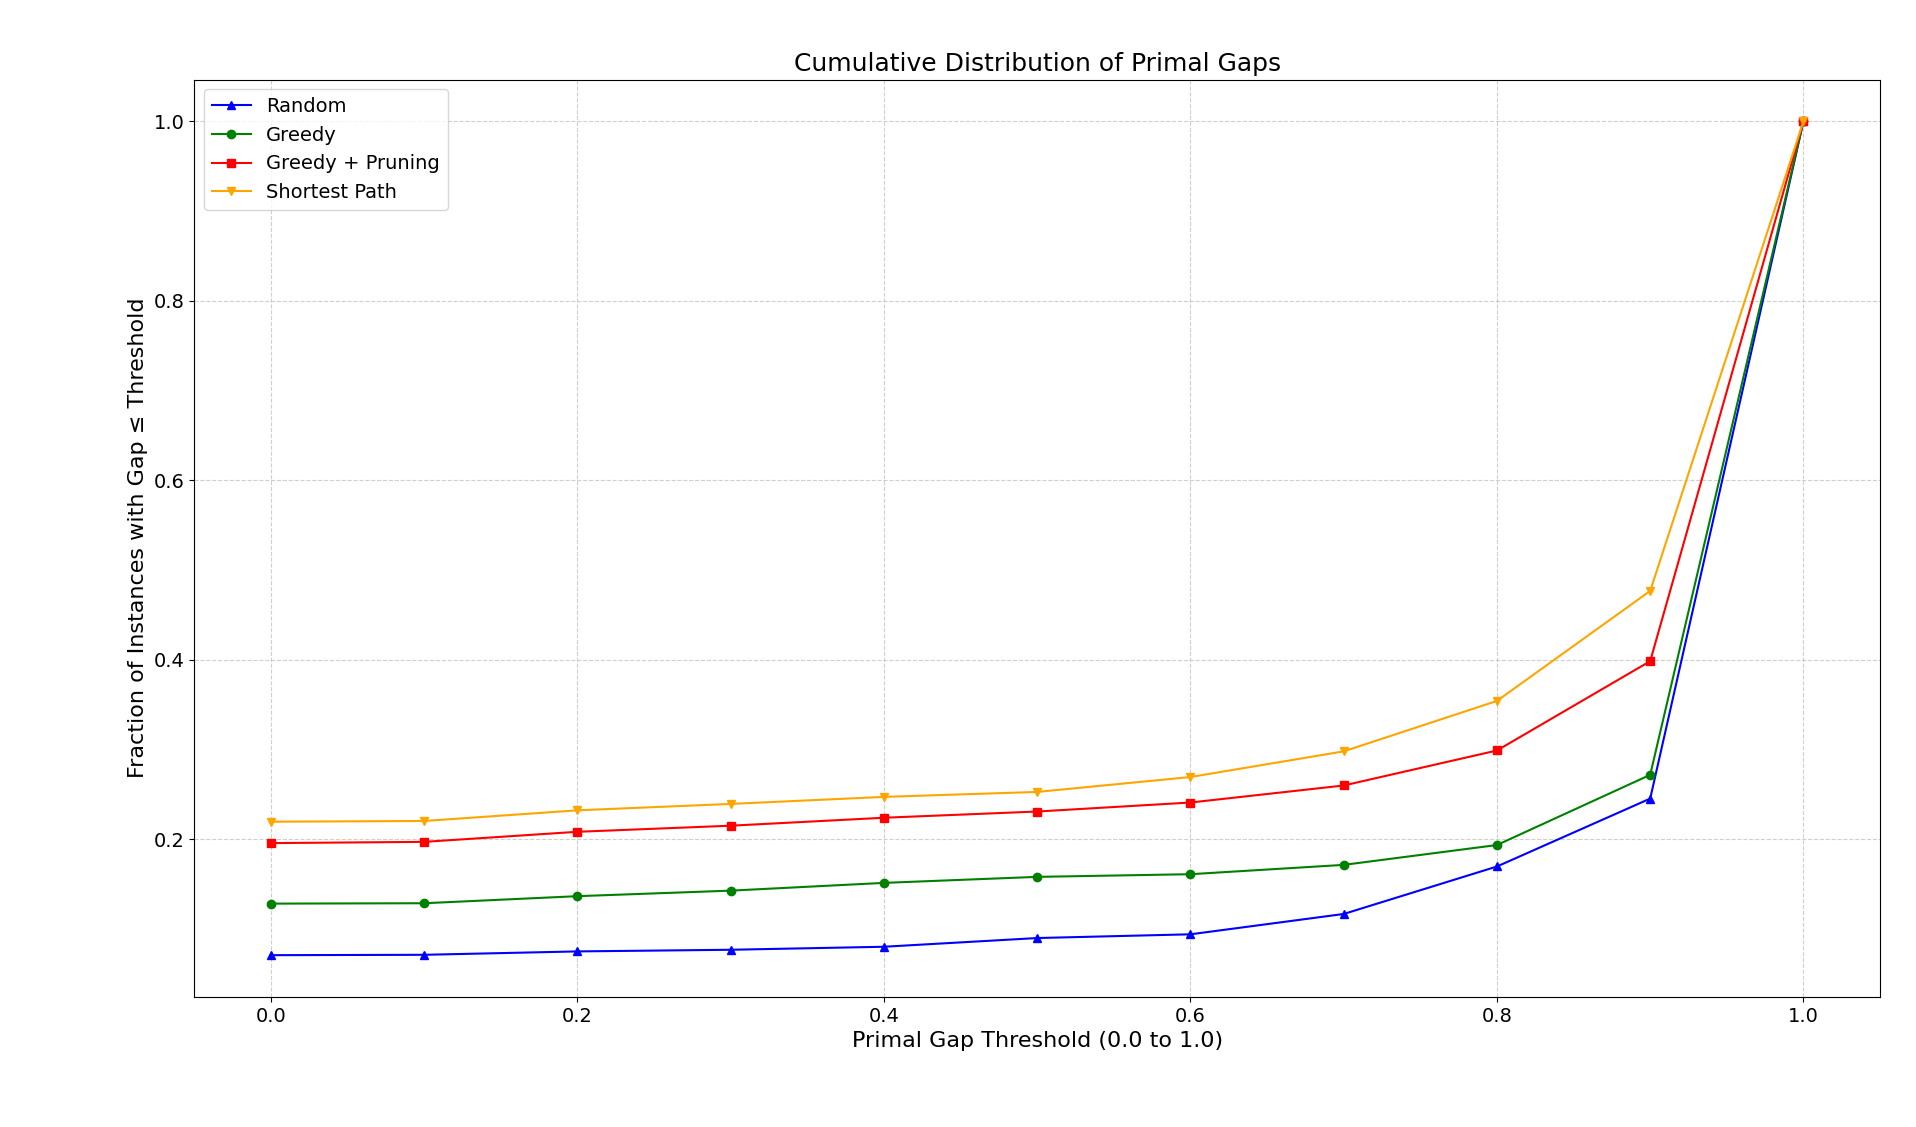
\includegraphics[width=\textwidth]{images/algs0124.png}
	\caption{Cumulative distribution plot for Random, Greedy, Greedy + Pruning, and Shortest Path strategies.}
	\label{fig:rgps}
\end{figure}

For instance, to better interpret the plot, consider the greedy strategy: the point on its curve corresponding to
a primal gap threshold of 60\% is close to 20\%. This indicates that it achieves a solution with a primal gap less than
or equal to 60\% in approximately 20\% of the problem instances.
Conversely, the shortest path strategy found the best known solution (i.e., a primal gap of 0\%) in approximately
25\% of the instances.
Now that the plot has been properly explained, it is possible to identify the most effective heuristic.
The curve that remains above all the others represents the best-performing strategy, as it indicates that the corresponding
algorithm consistently found solutions within the primal gap thresholds for a larger number of instances.
As expected, random and greedy stategies typically do not produce high-quality plans. Pruning the useless actions appears to be
an effective strategy, as it allows the planner to discard actions that are known to be unhelpful whenever multiple
options with the same cost are available.
Shortest Path builds on pruning by also estimating the distance to the goal for each action, resulting in a more
informed and effective selection of actions to include in the plan.

\section{Greedy + Pruning vs Hmax + Lookahead}
As shown in the previous section, pruning proves to be an effective strategy.
The initial idea was to combine pruning with the max heuristic. However, due to the nature of the heuristic’s definition,
this approach effectively reduces to a greedy + pruning strategy. To better evaluate its potential,
a lookahead mechanism was implemented to assess whether combining pruning with the max heuristic could lead
to a more promising solution. This section presents an evaluation of the performance of these two algorithms.
The lookahead process is computationally expensive; as a result, the algorithm fails to find a plan for approximately
one-third of the instances. Figure \ref{fig:algs23} presents the cumulative distribution plot comparing the performance
of these two algorithms.

\begin{figure}[ht]
	\centering
	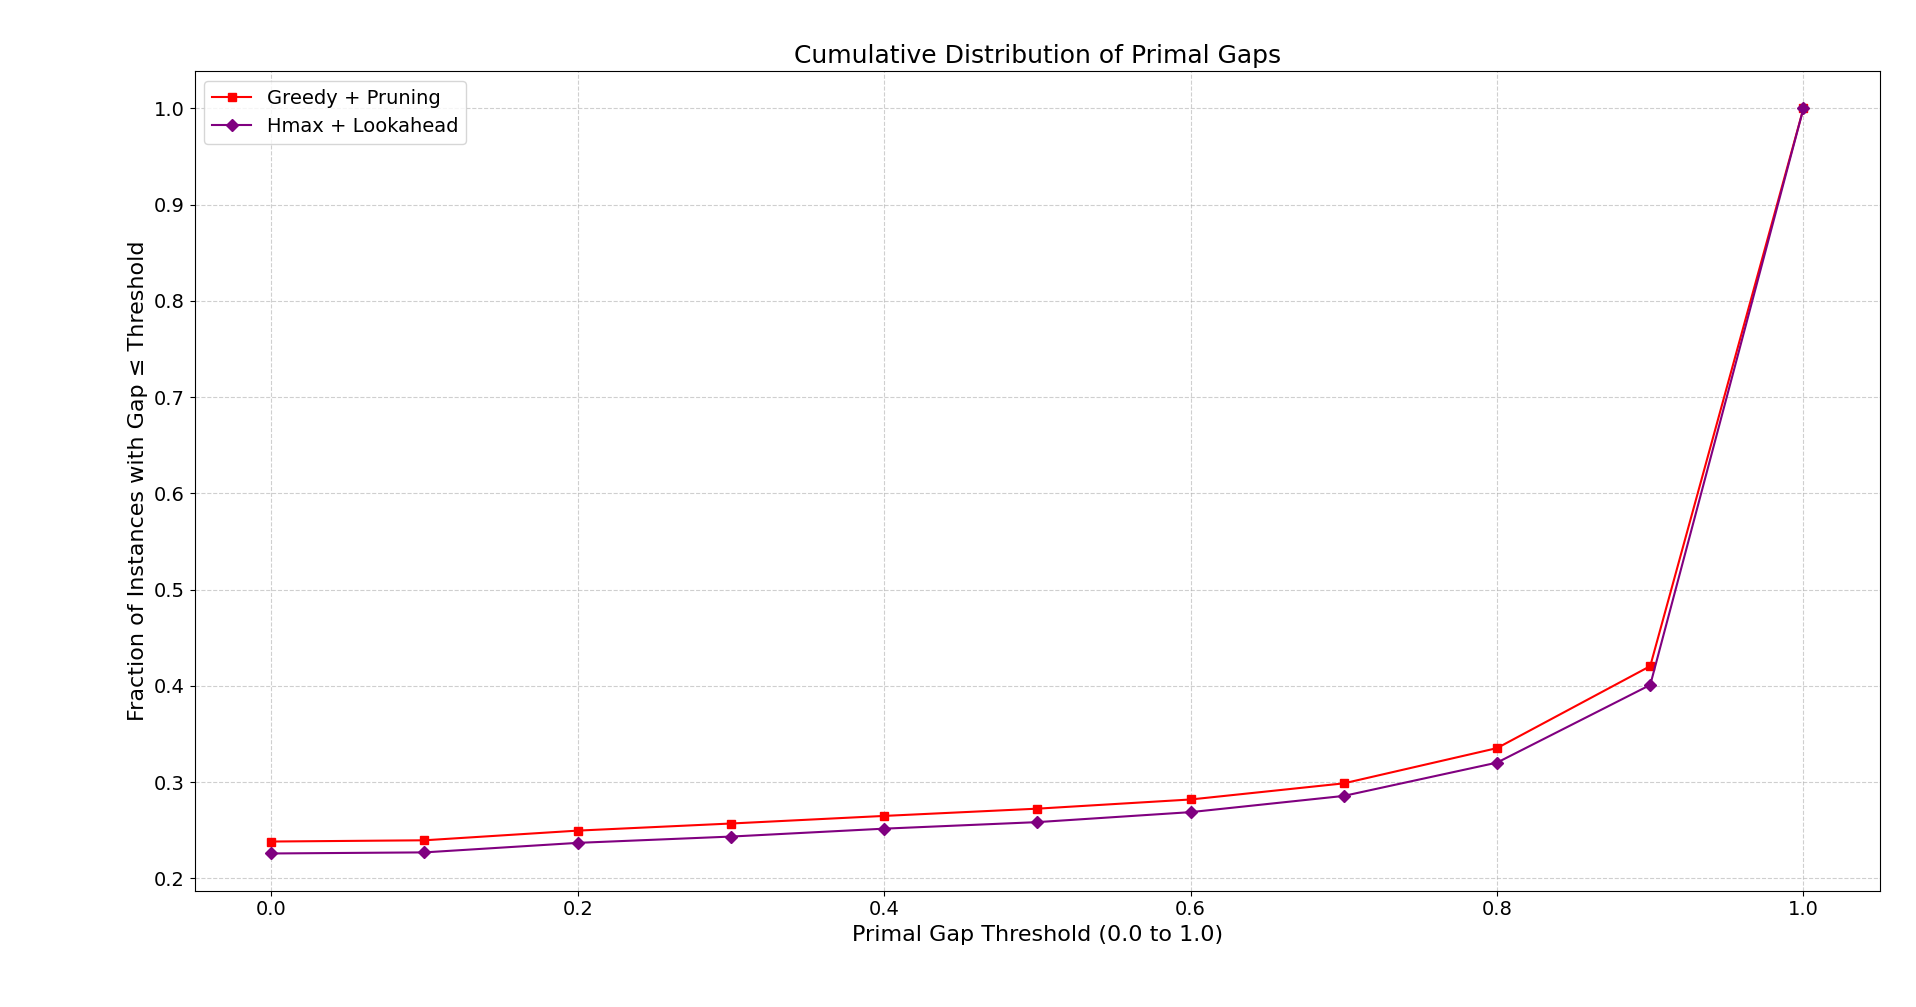
\includegraphics[width=\textwidth]{images/algs23.png}
	\caption{Cumulative distribution plot for Greedy + Pruning, and Max Heuristic + Lookahead strategies.}
	\label{fig:algs23}
\end{figure}

Unfortunately, this plot alone cannot definitively answer which of the two algorithms produces better-quality plans.
The high number of unsolved instances by the hmax + lookahead algorithm can skew the results: greedy + pruning may
appear superior simply because it solves more instances, not necessarily because it generates better plans.
There is no guarantee that the plans found by greedy + pruning are of higher quality than those returned by hmax + lookahead.
Figure \ref{fig:algs234_solved_all} shows a comparison between the algorithms, considering only the instances that were successfully
solved by all of them.

\begin{figure}[ht]
	\centering
	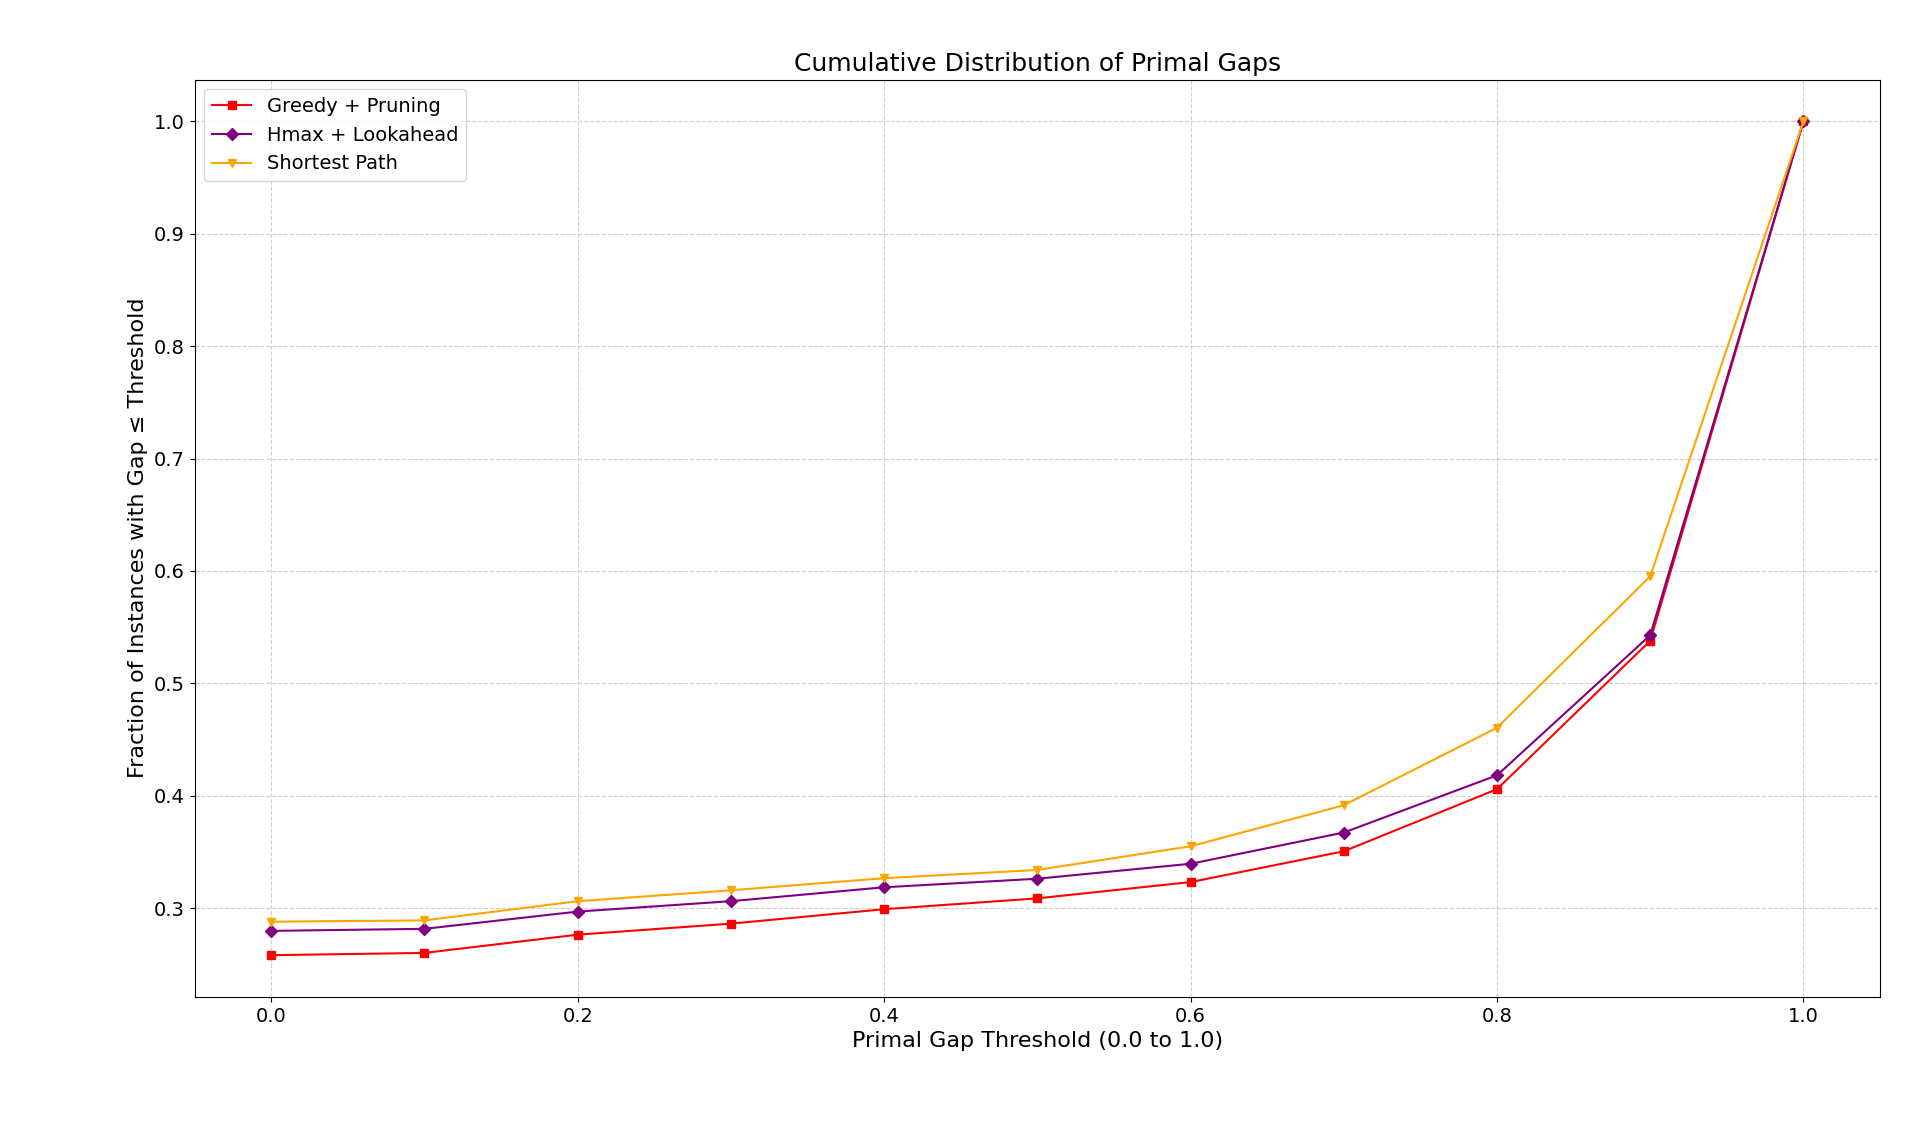
\includegraphics[width=\textwidth]{images/algs234_solved_all.png}
	\caption{Cumulative distribution plot for Greedy + Pruning, Max Heuristic + Lookahead, and Shortest Path strategies,
		considering only the instances solved by all of them.}
	\label{fig:algs234_solved_all}
\end{figure}

The curve for shortest path is included as a reference. Focusing only on the instances solved by all the presented algorithms
is particularly valuable: in this case, the curves are not skewed by instances that some strategies failed to solve.
This allows us to assess only the quality of the generated plans. From this comparison, it is evident that shortest path
is the best-performing algorithm overall—both in terms of solution quality and the number of problems it can solve.
Additionally, the performance of hmax + lookahead, which surpasses that of greedy + pruning, confirms that pruning combined
with max heuristic can be an effective strategy when paired with a lookahead mechanism.
Although lookahead remains a slow algorithm, these results suggest that the revised version of the max heuristic|enhanced
with a pruning mechanism|has the potential to produce high-quality solutions if used within a more powerful search strategy
like \verb|A*|.

\section{Different Versions of Backward Propagation}
As explained in Section \ref{sec:shortestpath}, the core idea behind the algorithm is to back-propagate the estimated cost
of reaching the goal state from its constituent facts to those in the current state. Previously, an algorithm was introduced
that propagates the minimum cost among an action's effects—effectively computing the shortest path to the goal.
With minimal modification, alternative strategies can be explored, such as propagating the \textit{maximum effect cost} or the
\textit{sum of all effect costs} to preceding actions. These variations are evaluated in Figure \ref{fig:backprop} to determine which
propagation strategy yields better results.

\begin{figure}[ht]
	\centering
	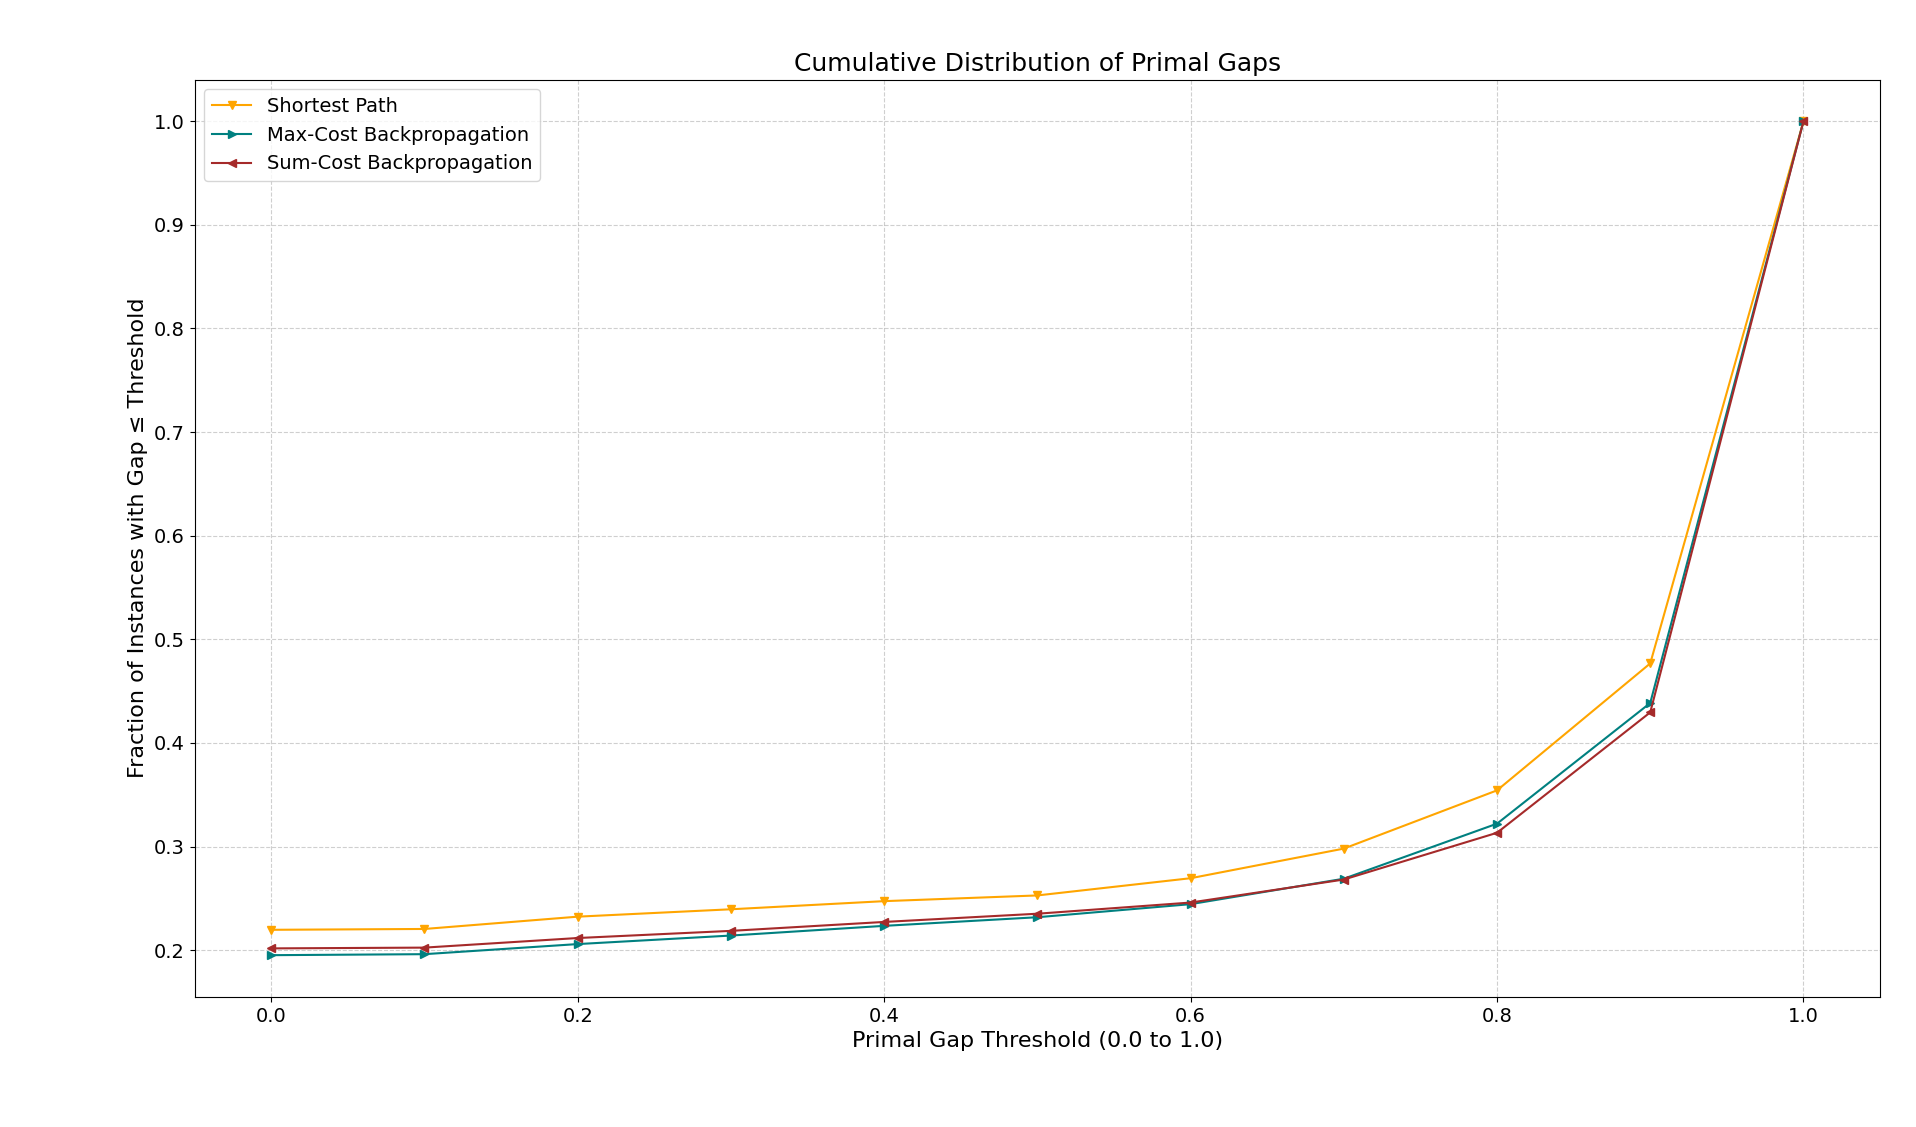
\includegraphics[width=\textwidth]{images/algs456.png}
	\caption{Cumulative distribution plot for different backpropagation strategies}
	\label{fig:backprop}
\end{figure}

Back-propagating the maximum cost among an action’s effects can be interpreted as assigning the action a cost based on
the worst-case path to the goal state. Conversely, back-propagating the sum of the effects' costs reflects a perspective
where all possible outcomes of the action contribute to estimating the distance to the goal. Each approach offers a different
trade-off between pessimism and comprehensiveness in cost estimation.
The Shortest Path heuristic continues to deliver the best performance overall. In contrast, both the max-cost and sum-cost
backpropagation strategies exhibit similar behavior, with only marginal differences between them.

\section{Randomization Analysis}
All the presented algorithms share a common trait: when multiple actions have the same minimum heuristic cost,
the next action is selected at random among them.
This section analyzes the impact of random tie-breaking on the quality of the returned plans. As mentioned earlier,
each algorithm was executed on every instance using 10 different random seeds. Varying the seed affects the algorithm’s
behavior only in cases where multiple actions share the same heuristic cost, influencing which action is selected among them.
Figure \ref{fig:rand_rand} presents the analysis of the impact of randomization on the random strategy.

\begin{figure}[ht]
	\centering
	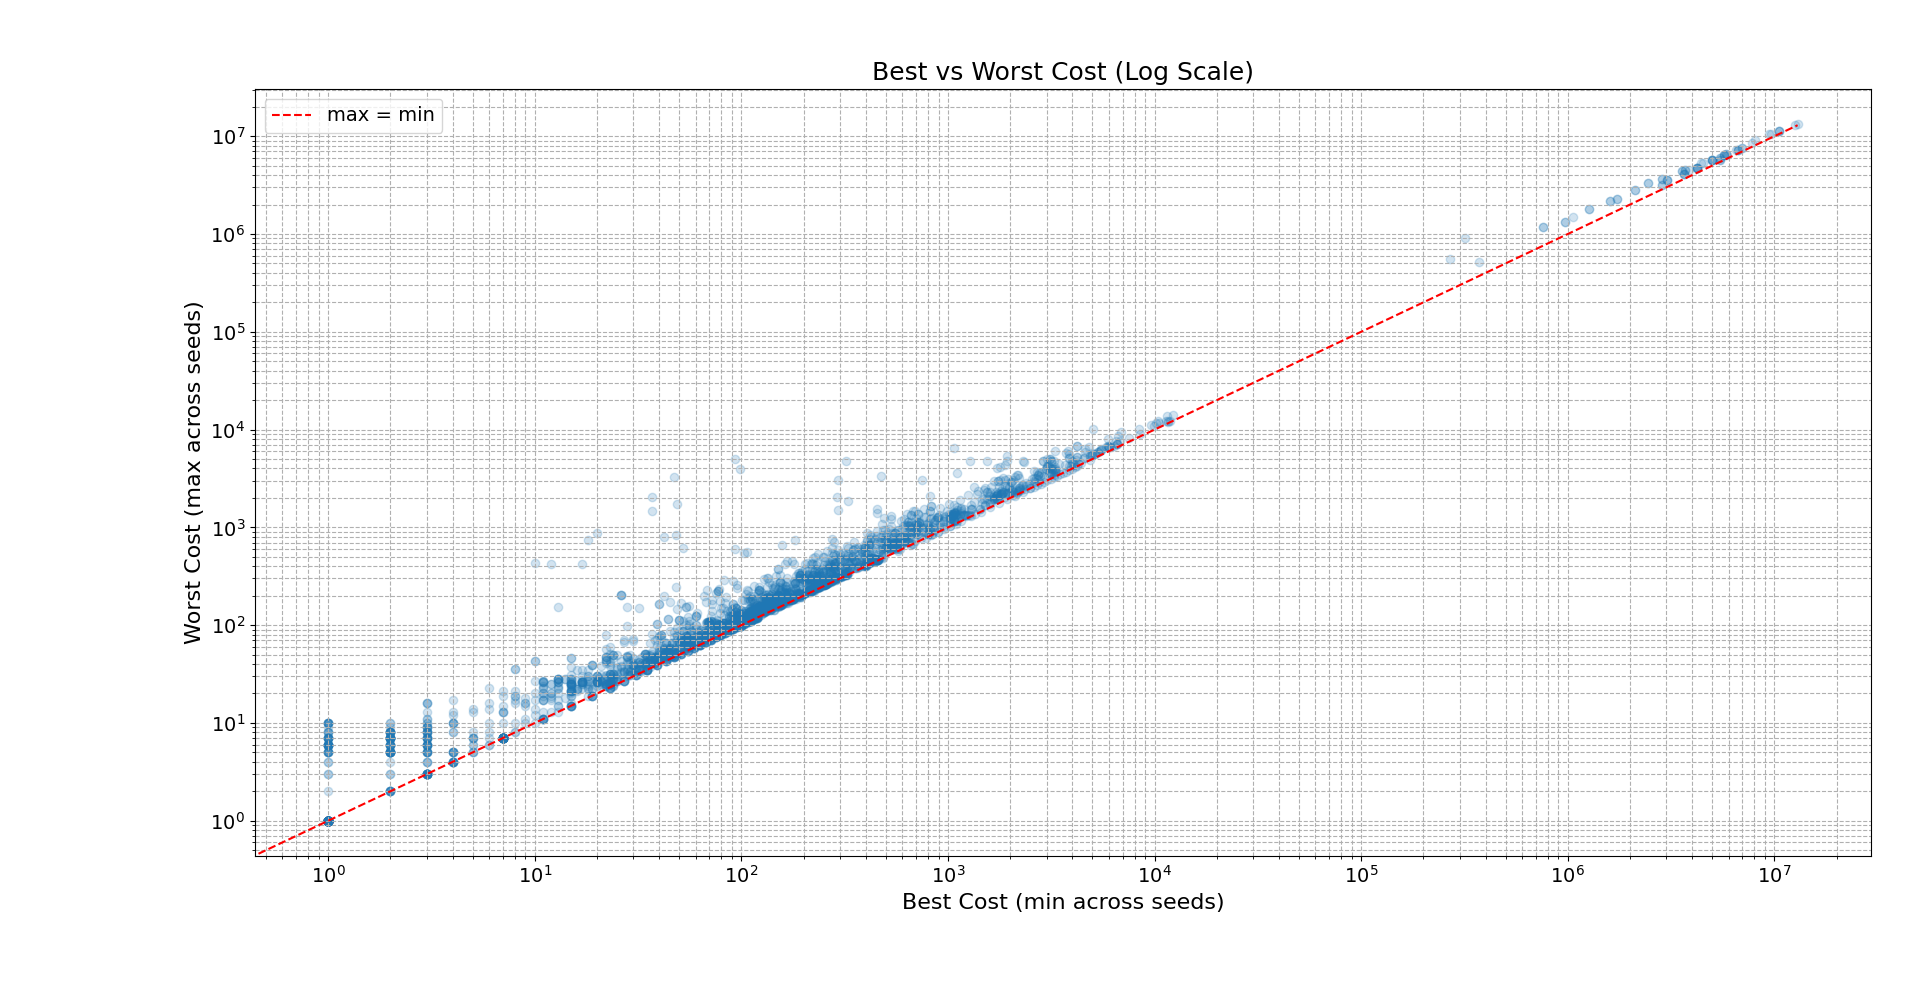
\includegraphics[width=\textwidth]{images/randomization_random.png}
	\caption{Effect of random seed on the outcome variability of the Random approach.}
	\label{fig:rand_rand}
\end{figure}

It is a \textit{logarithmic plot}: it uses a logarithmic scale on both axis to display data with a wide range of value.
Each point represents one instance in the testbed, and its coordinates correspond to the minimum and maximum plan costs found
by the algorithm across different random seeds.
Some instances exhibit a large discrepancy between the minimum and maximum plan costs. In fact, certain points show a minimum
cost of around 10 and a maximum close to 1000, indicating a fluctuation of two orders of magnitude.
Selecting the next action at random is highly dependent on the chosen random seed.
Figure \ref{fig:rand_greedy} shows the same plot for the greedy approach.

\begin{figure}[ht]
	\centering
	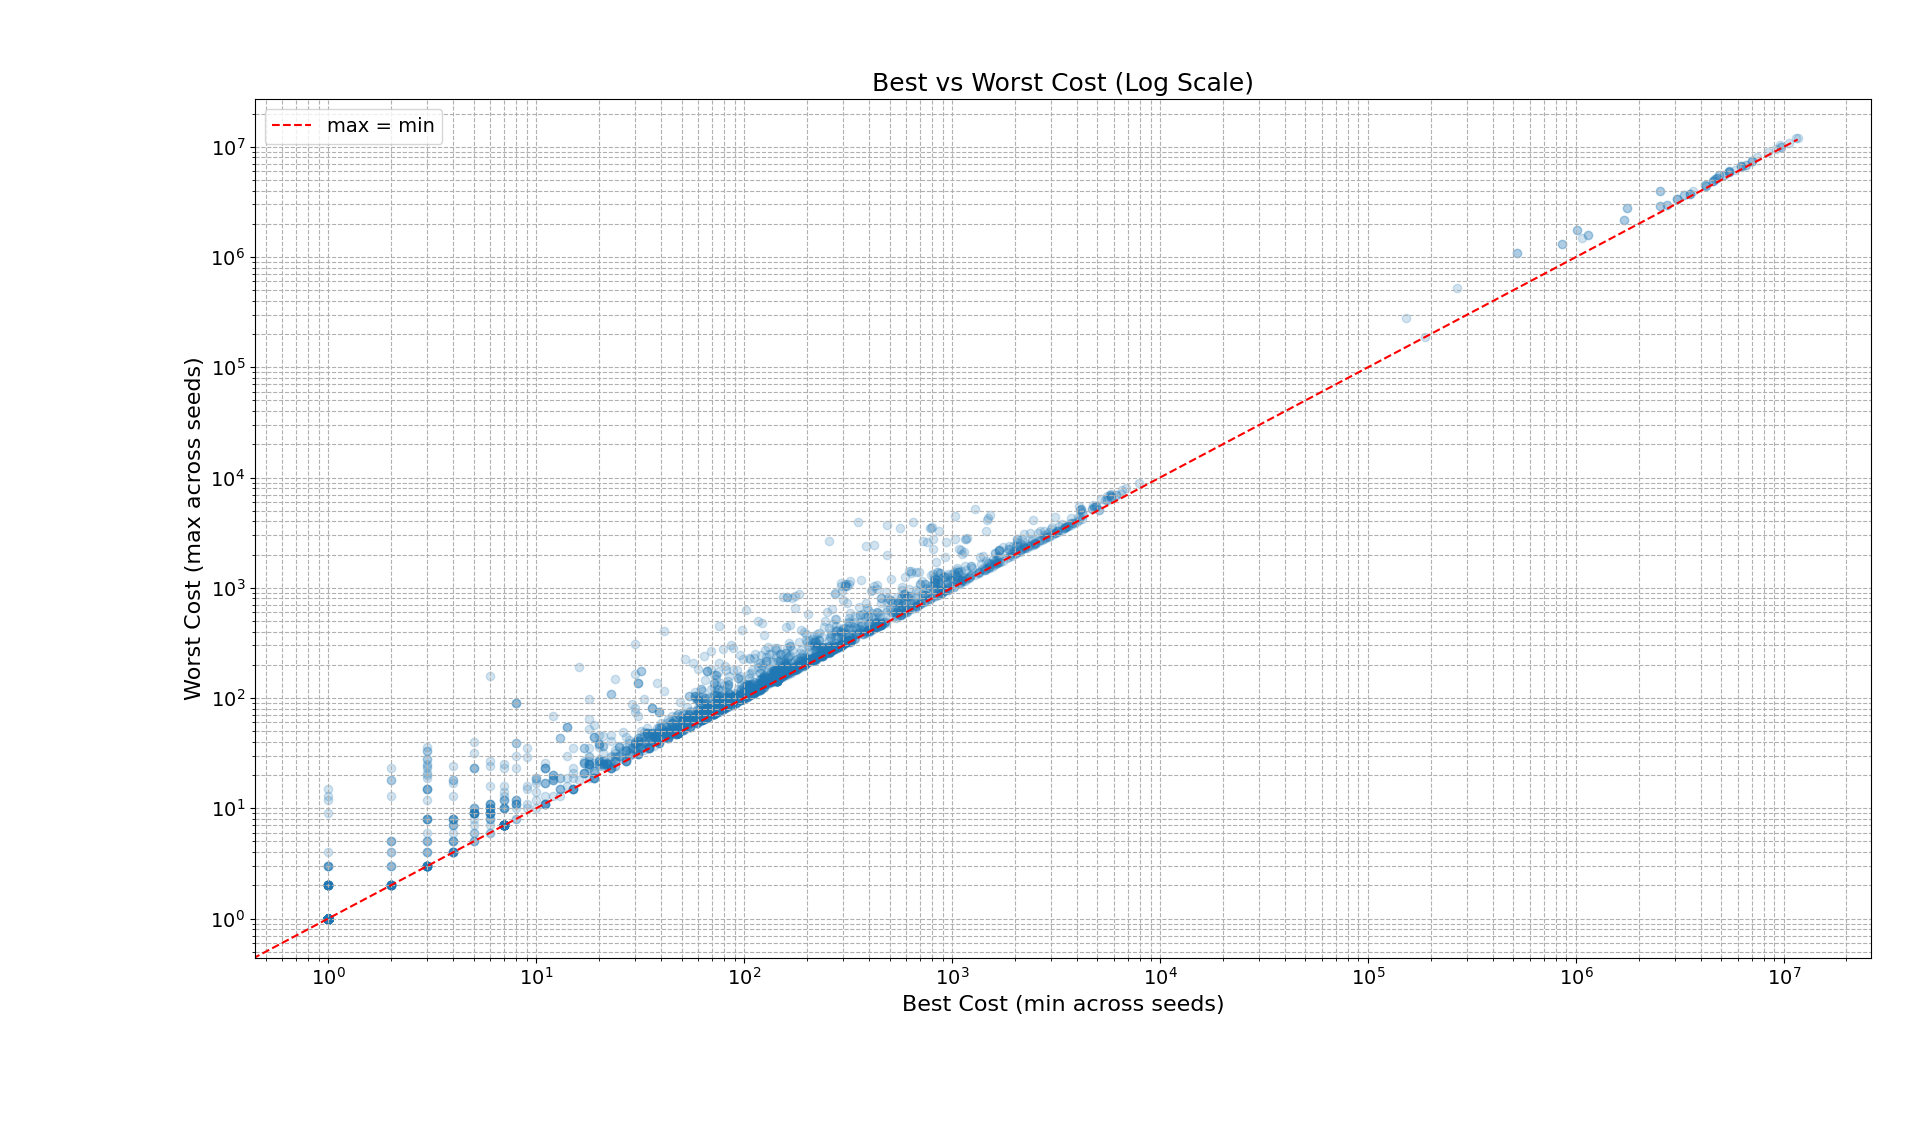
\includegraphics[width=\textwidth]{images/randomization_greedy.png}
	\caption{Effect of random seed on the outcome variability of the Greedy approach.}
	\label{fig:rand_greedy}
\end{figure}

In this case, the variability in the algorithm's output is more stable than in the previous one. While the greedy strategy still
exhibits instances with large discrepancies between minimum and maximum costs, both the frequency and the magnitude of these
differences are slightly reduced.
The overall trend emerging from this analysis is that the more informative the heuristic, the more stable its results become.
This behavior is particularly evident in Figures~\ref{fig:rand_pruning} and~\ref{fig:rand_sp}.

\begin{figure}[ht]
	\centering
	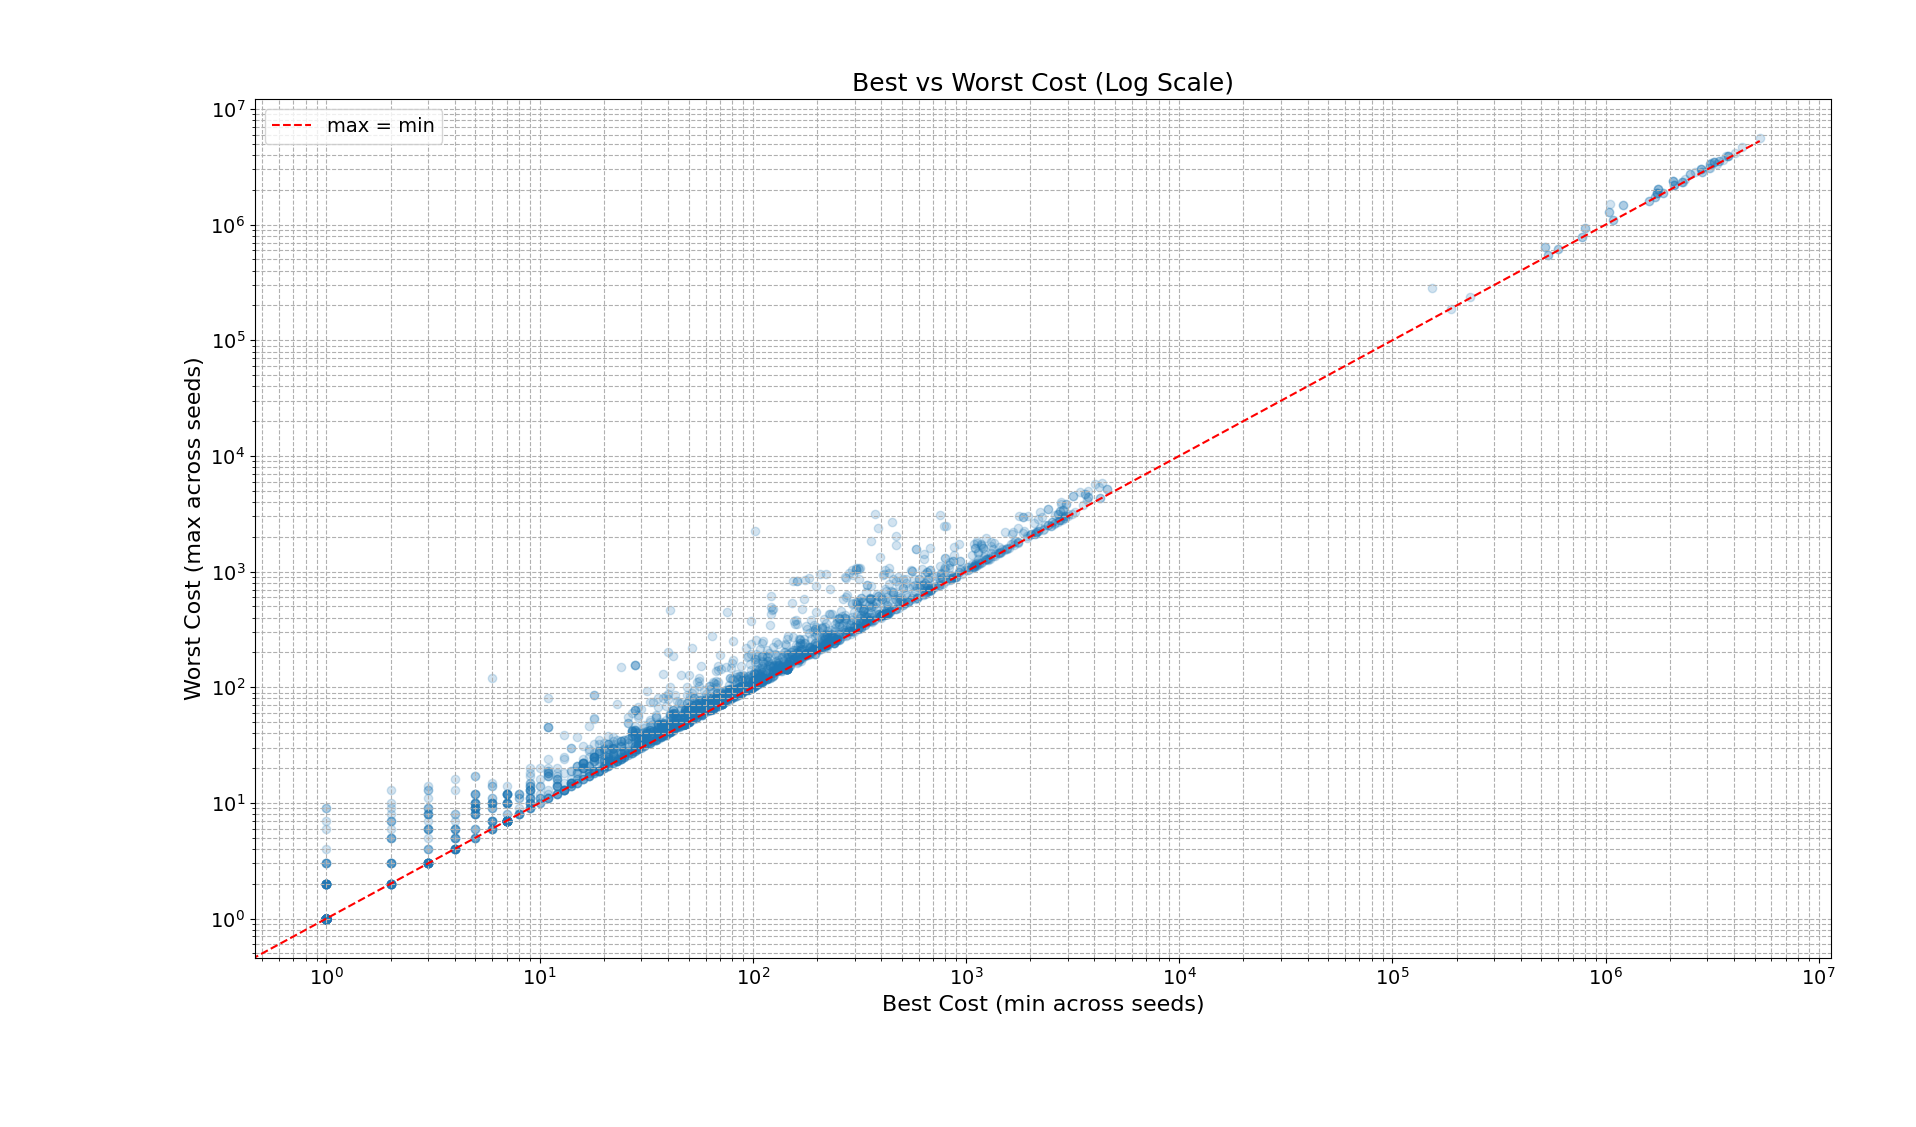
\includegraphics[width=\textwidth]{images/randomization_pruning.png}
	\caption{Effect of random seed on the outcome variability of the Greedy + Pruning approach.}
	\label{fig:rand_pruning}
\end{figure}

\begin{figure}[ht]
	\centering
	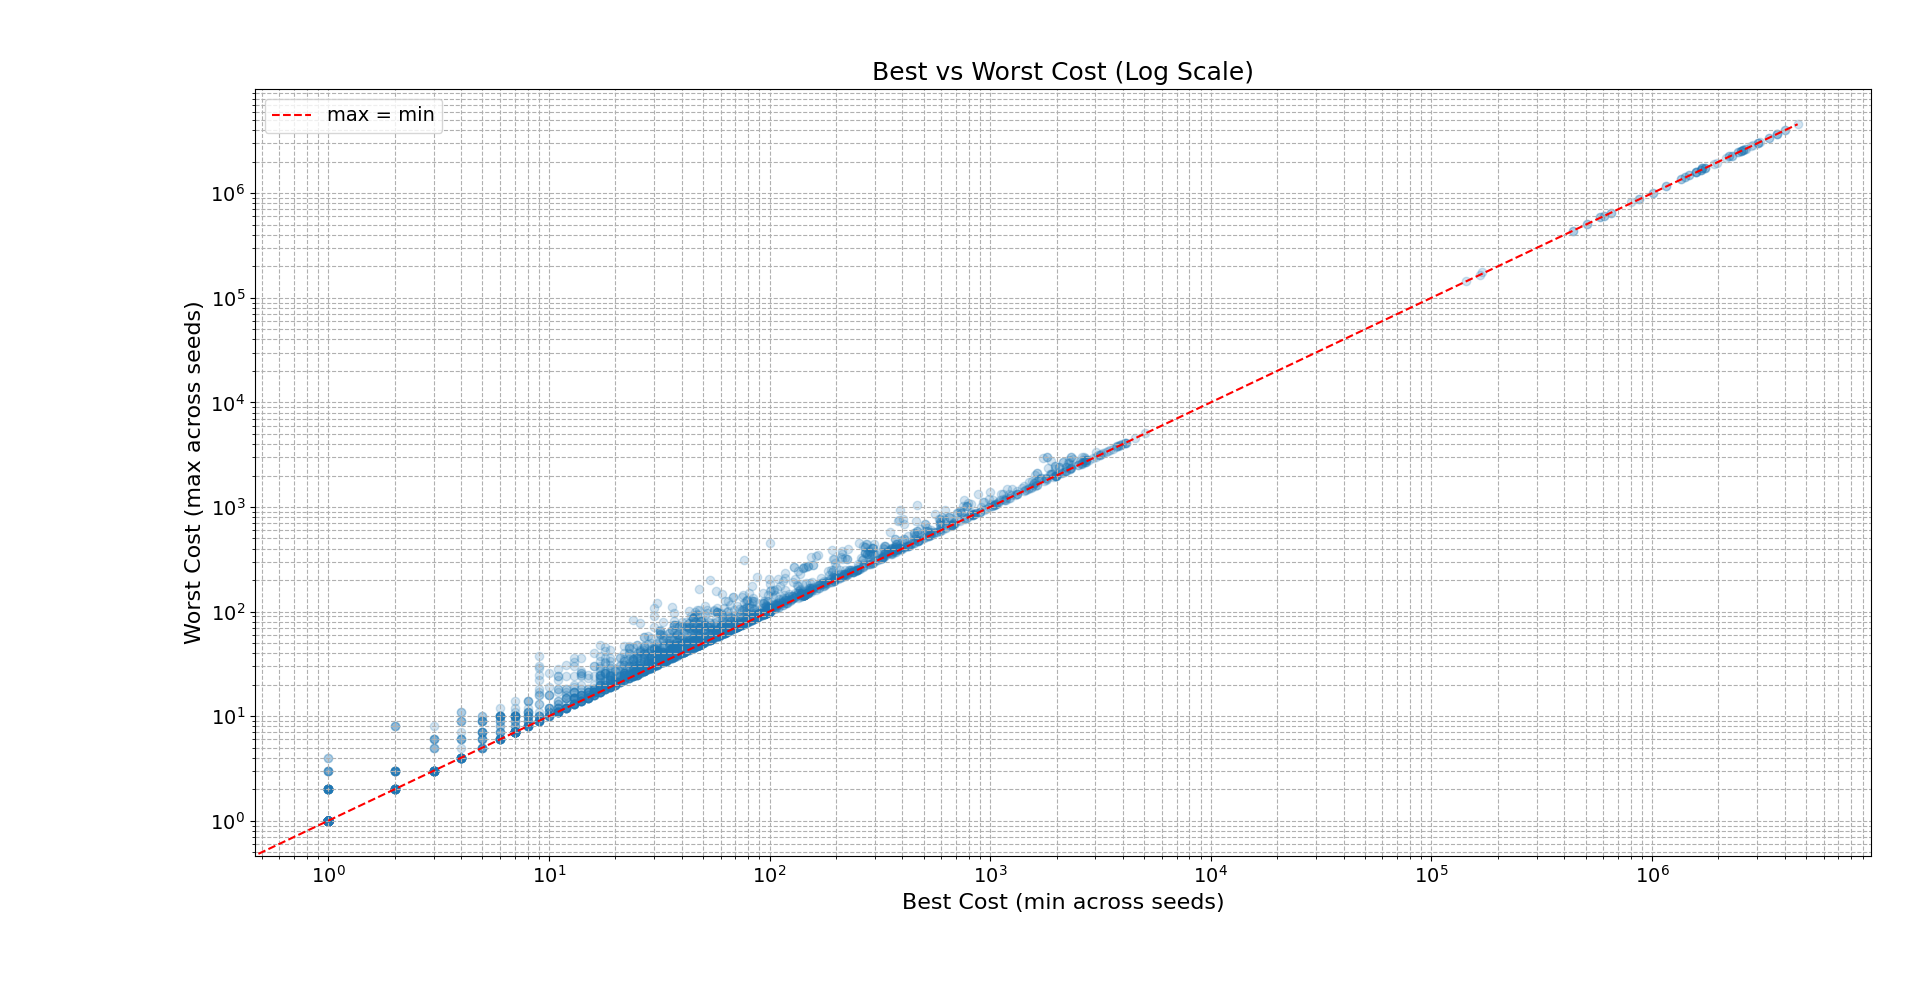
\includegraphics[width=\textwidth]{images/randomization_sp.png}
	\caption{Effect of random seed on the outcome variability of the Shortest Path approach.}
	\label{fig:rand_sp}
\end{figure}

The improvement is especially noticeable in the plot for the shortest path heuristic. Most points lie close to the red line,
which represents the ideal case where the minimum and maximum plan costs are equal. This indicates a high degree of consistency
across different random seeds. The shortest path approach stands out as the most informative among the heuristics presented,
combining a pruning mechanism with an action-level estimate of the distance to the goal state.\\
In conclusion, the shortest path heuristic proves to be the most effective in all aspects: it solves the largest number of instances,
yields the best performance in cumulative distribution plots, and demonstrates the highest stability with respect to random seed variation.

\section{Iterative Refinement via Shortest Path Reapplication}
In the context of Mixed Integer Programming (MIP), there is a technique known as \textit{local branching} \cite{fischetti2003local},
which involves first finding a feasible solution using a fast heuristic or metaheuristic approach, and then refining this solution by solving,
to optimality, a subproblem of the original MIP using a solver as a ``black box''.
This approach could also be applied to planning. However, at the time of writing, the most well-known optimal planner, Fast Downward,
does not provide an API that would allow it to be used as a black-box component. To refine the solution found by the shortest path heuristic,
the proposed idea is to reapply the algorithm to a subproblem and then replace the corresponding segment of the original solution with the new one.
The hope is that solving a smaller, focused subproblem may yield a higher-quality solution than addressing the full problem in its entirety.
Given an initial plan, the initial and goal states for the subproblem are derived from intermediate states along the original plan.
In the experiment, these subproblem boundaries were positioned at different segments of the original solution.
For each instance, the shortest path algorithm was reapplied to three different segments of the original plan: the first 30\% of actions,
the central 40\%, and the final 30\%.
The original segments of the solution were replaced with the newly generated ones, and the total plan cost was then recomputed.
If the new cost is better than the initial one, the new solution is returned; otherwise, the initial solution is retained as the final plan.
Figure \ref{fig:reapply} compares the cumulative distribution of the original shortest path
strategy with the three variants where the algorithm was reapplied to different segments of the plan.

\begin{figure}[ht]
	\centering
	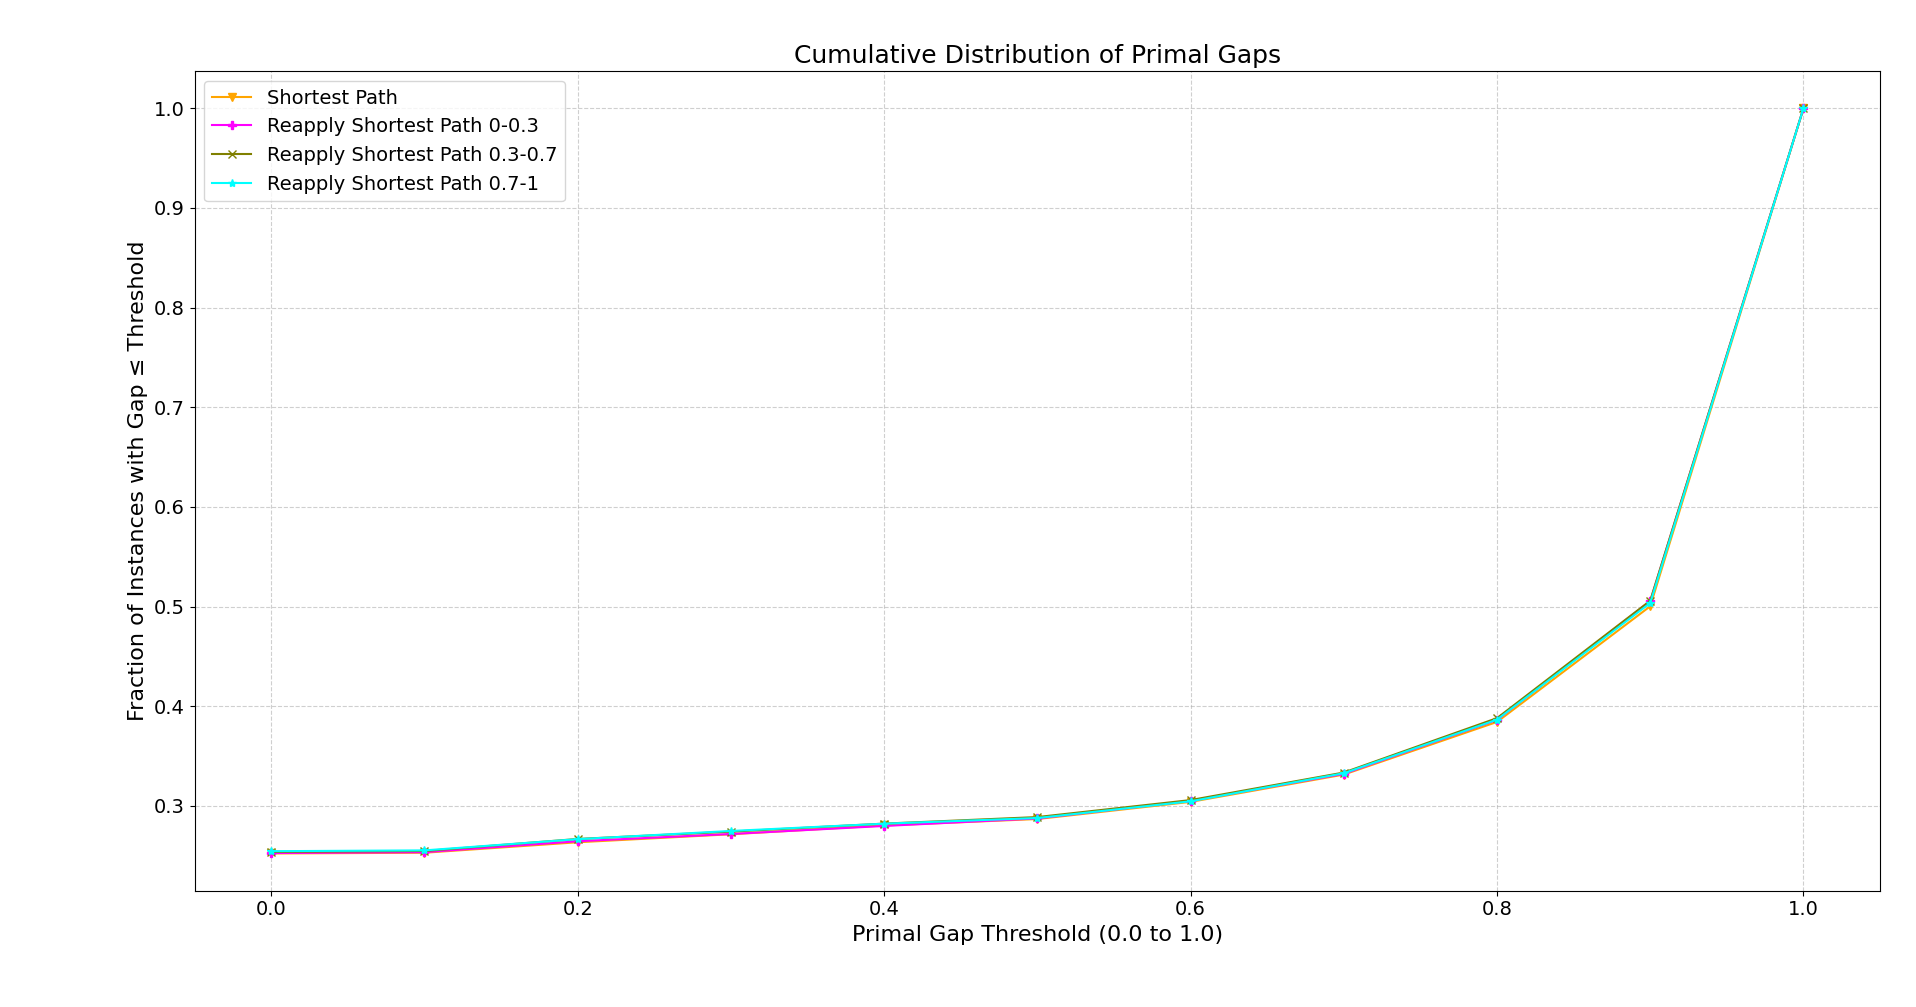
\includegraphics[width=\textwidth]{images/reapply_full.png}
	\caption{Comparison of cumulative distributions for Shortest Path reapplied to different plan segments.}
	\label{fig:reapply}
\end{figure}

Unfortunately, the four curves overlap almost entirely, indicating that this strategy yields only minimal refinement over the initial solution.
While the cost of the refined plans may occasionally differ from the original, the improvements are generally negligible.
This suggests that reapplying the heuristic to subproblems does not significantly enhance solution quality and may not be an effective
refinement approach in practice.

\section{Iterative Refinement via Uniform Cost Search}
In the previous section, an analysis was conducted on refining the solution provided by the shortest path heuristic by reapplying the same method
to different segments of the original plan.
Now, a different approach is explored by using \textit{Uniform Cost Search (UCS)} \cite{felner2011position} as the refinement algorithm.
\verb|UCS| is an exact algorithm that always finds the optimal path from a starting node to a goal node in a graph.
It maintains a priority queue to track the frontier of nodes that have not yet been expanded. A node is considered expanded once all of its
neighbors have been discovered.
At each iteration, the node with the lowest cost—defined as the actual cost incurred to reach it from the starting node—is extracted from the queue.
By always expanding the node with the minimum cost, \verb|UCS| guarantees that the solution returned is optimal.
Algorithm \ref{alg:ucs} presents the pseudocode for this strategy.

\begin{algorithm}
	\caption{Uniform Cost Search}
	\label{alg:ucs}
	\hspace*{0.5em} \textbf{Output}: optimal plan
	\begin{algorithmic}[1]
		\Procedure{ucs}{$planningTask$}
		\State $stateCosts \gets \{+\infty, \dots, +\infty\}$ \Comment{Initialize states' cost to $+\infty$}
		\State $pq \gets \{\}$ \Comment{Empty priority queue}
		\State $visited \gets \{\}$ \Comment{Empty visited set}
		\State $stateCosts[planningTask.initialState] \gets 0$
		\State $\Call{push}{pq, planningTask.initialState, 0}$ \Comment{Push the initial state with cost 0}
		\While {$!\Call{empty}{pq}$}
		\State $state \gets \Call{pop}{pq}$ \Comment{Get the state having minimum cost}
		\If {$planningTask.goalState \subseteq state$}
		\State \textbf{return} \Call{extractPlan}{state}
		\EndIf
		\If {$state \in visited$}
		\State $continue$ \Comment{Skip already expanded states}
		\EndIf
		\State $visited \gets visited \cup \{state\}$
		\State $successors \gets \{a \in A \mid pre(a) \subseteq state\}$
		\ForAll {$action \in successors$}
		\State $nextState \gets \Call{apply}{state, action}$
		\State $newCost \gets action.cost + stateCosts[state]$
		\If {$newState \notin visited \textbf{ and } newCost < stateCosts[newState]$}
		\State $stateCosts[newState] \gets newCost$
		\If {$\Call{has}{pq, newState}$}
		\State $\Call{change}{pq, newState, newCost}$
		\Else
		\State $\Call{push}{pq, newState, newCost}$
		\EndIf
		\EndIf
		\EndFor
		\EndWhile
		\EndProcedure
	\end{algorithmic}
\end{algorithm}
